\documentclass[DaoFP]{subfiles}
\begin{document}
\setcounter{chapter}{11}

\chapter{余代数}

余代数(Coalgebras)只是对偶范畴中的代数。本章结束!

好吧,也许还没完...正如我们之前所见,我们所工作的范畴在对偶性方面并不对称。特别是,如果我们比较终对象和始对象,它们的性质并不对称。我们的始对象没有进入的箭头,而终对象除了有唯一的进入箭头外,还有许多出去的箭头。

由于始代数是从始对象开始构造的,我们可能会期望终余代数——它们是始代数的对偶,因此从终对象生成——不仅仅是它们的镜像,而是会添加它们自己有趣的变化。

我们已经看到,代数的主要应用是处理递归数据结构:在折叠它们时。对偶地,余代数的主要应用是生成或展开递归的、树状的数据结构。展开是使用变形(anamorphism)完成的。

我们使用折叠(catamorphism)来砍树,我们使用变形来种树。

我们不能无中生有地产生信息,因此一般来说,折叠和变形都倾向于减少其输入中包含的信息量。

在你对一个整数列表求和后,无法恢复原始列表。

同样地,如果你使用变形生成一个递归数据结构,种子必须包含最终出现在树中的所有信息。你不会获得新的信息,但优势在于你现在拥有的信息以一种更方便进一步处理的形式存储。

\section{自函子的余代数}

自函子 $F$ 的余代数是一个由载体 $a$ 和结构映射组成的对:一个箭头 $a \to F a$。

在 Haskell 中,我们定义:
\begin{haskell}
 type Coalgebra f a = a -> f a
\end{haskell}
我们通常将载体视为种子的类型,从中我们可以生成数据结构,无论是列表还是树。

例如,这里有一个可以用来创建二叉树的函子,整数存储在节点中:
\begin{haskell}
data TreeF x = LeafF | NodeF Int x x
  deriving (Show, Functor)
\end{haskell}
我们甚至不必为它定义 \hask{Functor} 的实例——\hask{deriving} 子句告诉编译器为我们生成规范的实例(连同 \hask{Show} 实例,如果我们想显示它,允许转换为 \hask{String})。

余代数是一个函数,它接受载体类型的种子并生成一个充满新种子的函子。这些新种子可以递归地用于生成子树。

这是函子 \hask{TreeF} 的一个余代数,它接受一个整数列表作为种子:
\begin{haskell}
split :: Coalgebra TreeF [Int]
split [] = LeafF
split (n : ns) = NodeF n left right
  where
    (left, right) = partition (<= n) ns
\end{haskell}
如果种子为空,它生成一个叶子;否则它创建一个新节点。该节点存储列表的头部,并用两个新种子填充节点。库函数 \hask{partition} 使用用户定义的谓词(这里是 \hask{(<= n)},小于或等于 \hask{n})拆分列表。结果是一对列表:第一个满足谓词;第二个不满足。

你可以确信,递归应用这个余代数会创建一个二叉排序树。我们稍后将使用这个余代数来实现排序。

\section{余代数的范畴}

通过与代数同态的类比,我们可以将余代数同态定义为满足交换条件的载体之间的箭头。

给定两个余代数 $(a, \alpha)$ 和 $(b, \beta)$,箭头 $f \colon a \to b$ 是一个余代数同态,如果下面的图表交换:

\[
 \begin{tikzcd}
 a 
 \arrow[r, "f"]
 \arrow[d, "\alpha"]
 & b
\arrow[d, "\beta"]
 \\
F  a
 \arrow[r, "F f"]
 & F b
  \end{tikzcd}
\]

其解释是,无论我们是先映射载体然后应用余代数 $\beta$,还是先应用余代数 $\alpha$ 然后使用提升 $F f$ 将箭头应用于其内容,结果都是相同的。

余代数同态可以组合,且恒等箭头自动是一个余代数同态。很容易看出,余代数与代数一样,形成了一个范畴。

然而,这次我们感兴趣的是这个范畴中的终端对象——\emph{终端余代数}。如果存在一个终端余代数 $(t, \tau)$,它满足Lambek引理的对偶。

\begin{exercise}{Lambek引理:}
证明终端余代数 $(t, \tau)$ 的结构映射 $\tau$ 是一个同构。提示:证明与初始代数的证明对偶。
\end{exercise}

作为Lambek引理的一个结果,终端代数的载体是所讨论的自函子的一个不动点。
\[ F t \cong t \]
其中 $\tau$ 和 $\tau^{-1}$ 作为这个同构的见证。

同样可以得出 $(t, \tau^{-1})$ 是一个代数;正如 $(i, \iota^{-1})$ 是一个余代数,假设 $(i, \iota)$ 是初始代数。

我们之前已经看到,初始代数的载体是一个不动点。原则上,同一个自函子可能有许多不动点。初始代数是最小不动点,而终端余代数是最大不动点。

自函子 $F$ 的最大不动点记为 $\nu F$,因此我们有:
\[ t = \nu F \]

我们还可以看到,从初始代数到终端余代数必须存在唯一的代数同态(一个catamorphism)。这是因为终端余代数也是一个代数。

类似地,从初始代数(也是一个余代数)到终端余代数存在唯一的余代数同态。事实上,可以证明在这两种情况下,它是相同的底层同态 $\rho \colon \mu F \to \nu F$。

在集合范畴中,初始代数的载体集是终端余代数的载体集的一个子集,函数 $\rho$ 将前者嵌入后者。
\[
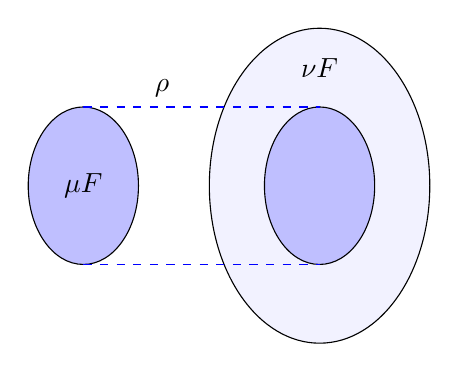
\begin{tikzpicture}
         \draw (-1,0)[fill=blue!25!white] ellipse (0.7 and 1);
         \draw (2,0)[fill=blue!5!white] ellipse (1.4 and 2);
         \draw (2,0)[fill=blue!25!white] ellipse (0.7 and 1);
         \node[above] at (0, 1) {$\rho$};
       	\draw[dashed, blue] (-1, 1) -- (2, 1);
	\draw[dashed, blue] (-1, -1) -- (2, -1);
        \node at (-1, 0) { $\mu F$ };
        \node at (2, 1.5) { $\nu F$ };
\end{tikzpicture}
\]

我们稍后会看到,在Haskell中,由于惰性求值,情况更加微妙。但是,至少对于具有叶子分量的函子——即它们在初始对象上的作用是非平凡的——Haskell的不动点类型既可以作为初始代数的载体,也可以作为终端余代数的载体。
\begin{haskell}
data Fix f where
  In :: f (Fix f) -> Fix f
\end{haskell}

\begin{exercise}
证明,对于 $\mathbf{Set}$ 中的恒等函子,每个对象都是一个不动点,空集是最小不动点,单例集是最大不动点。提示:最小不动点必须有箭头指向所有其他不动点,而最大不动点必须有箭头来自所有其他不动点。
\end{exercise}

\begin{exercise}
证明空集是 $\mathbf{Set}$ 中恒等函子的初始代数的载体。对偶地,证明单例集是这个函子的终端余代数。提示:证明唯一的箭头确实是(余)代数同态。
\end{exercise}

\section{变形(Anamorphisms)}

终余代数(terminal coalgebra) $(t, \tau)$ 由其泛性质定义:对于任何余代数 $(a, \alpha)$,存在唯一的余代数态射 $h$ 到 $(t, \tau)$。这个态射被称为\emph{变形(anamorphism)}。作为余代数态射,它使得以下图表交换:
\[
 \begin{tikzcd}
 a 
 \arrow[r, dashed, "h"]
 \arrow[d, "\alpha"]
 & t
\arrow[d, "\tau"]
 \\
 F a
 \arrow[r,  "F h"]
 & F t
  \end{tikzcd}
\]
 
 就像代数的情况一样,我们可以使用Lambek引理来“求解” \hask{h}:
 \[ h = \tau^{-1} \circ F h \circ \alpha \]
 这个解被称为变形,有时使用\index{透镜括号}\index{$\llens \rlens$}“透镜括号”表示为 $\llens \alpha \rlens$。
 
 由于终余代数(就像初始代数)是函子的不动点,上述递归公式可以直接翻译为Haskell代码:
 \begin{haskell}
ana :: Functor f => Coalgebra f a -> a -> Fix f
ana coa = In . fmap (ana coa) . coa 
\end{haskell}
这个公式的解释如下:给定一个类型为 \hask{a} 的种子,我们首先用余代数 \hask{coa} 作用于它。这给我们提供了一组种子。我们通过递归地应用变形来扩展这些种子,使用 \hask{fmap}。然后我们应用构造函数 \hask{In} 来得到最终结果。
 
作为一个例子,我们可以将变形应用于之前定义的 \hask{split} 余代数:\hask{ana split} 接受一个整数列表并创建一个排序树。

然后我们可以使用一个变形(catamorphism)将这个树折叠成一个排序列表。我们定义以下代数:
\begin{haskell}
toList :: Algebra TreeF [Int]
toList LeafF = []
toList (NodeF n ns ms) = ns ++ [n] ++ ms
\end{haskell}
它将左列表与单元素枢轴和右列表连接起来。为了对列表进行排序,我们将变形与变形结合:
\begin{haskell}
qsort = cata toList . ana split
\end{haskell}
这为我们提供了一个(非常低效的)快速排序实现。我们将在下一节中再次讨论它。

\subsection{无限数据结构}

在研究代数时,我们依赖于具有叶子组件的数据结构——即作用于初始对象时会产生不同于初始对象的结果的自函子。在构造递归数据结构时,我们必须从某个地方开始,这意味着首先构造叶子。

对于余代数,我们可以自由地放弃这一要求。我们不再需要“手动”构造递归数据结构——我们有变形来为我们完成这项工作。没有叶子的自函子是完全可以接受的:它的余代数将生成无限数据结构。

由于Haskell的惰性,无限数据结构是可表示的。事物是根据需要来评估的。只有那些明确需要的无限数据结构部分才会被计算;其余部分的评估保持在暂停状态。

在严格的语言中实现无限数据结构,必须将值表示为函数——这是Haskell在幕后所做的(这些函数被称为\emph{thunks})。

让我们看一个简单的例子:一个无限的值流。为了生成它,我们首先定义一个函子,它看起来非常像我们用来生成列表的函子,只是它缺少叶子组件(空列表构造函数)。你可能会认出它是一个积函子,第一个组件固定为流的有效载荷:
\begin{haskell}
data StreamF a x = StreamF a x
  deriving Functor
\end{haskell}
无限流是这个函子的不动点。
\begin{haskell}
type Stream a = Fix (StreamF a)
\end{haskell}
这里是一个简单的余代数,它使用一个整数 \hask{n} 作为种子:
\begin{haskell}
step :: Coalgebra (StreamF Int) Int
step n = StreamF n (n+1)
\end{haskell}
它将当前种子存储为有效载荷,并用 \hask{n + 1} 作为下一个流的种子。

当以零为种子时,这个余代数的变形生成所有自然数的流。
\begin{haskell}
allNats :: Stream Int
allNats = ana step 0
\end{haskell}
在非惰性语言中,这个变形将永远运行,但在Haskell中它是即时的。增量代价仅在我们想要检索某些数据时支付,例如,使用这些访问器:
\begin{haskell}
head :: Stream a -> a
head (In (StreamF a _)) = a

tail :: Stream a -> Stream a
tail (In (StreamF _ s)) = s
\end{haskell}

\section{合态射(Hylomorphisms)}

同态射(anamorphism)的输出类型是函子的不动点,这与归约态射(catamorphism)的输入类型相同。在Haskell中,它们都由相同的数据类型\hask{Fix f}描述。因此,可以将它们组合在一起,就像我们在实现快速排序时所做的那样。事实上,我们可以将余代数(coalgebra)与代数(algebra)结合在一个递归函数中,称为\emph{合态射(hylomorphism)}:
\begin{haskell}
hylo :: Functor f => Algebra f b -> Coalgebra f a -> a -> b
hylo alg coa = alg . fmap (hylo alg coa) . coa 
\end{haskell}
我们可以将快速排序重写为合态射:
\begin{haskell}
qsort = hylo toList split
\end{haskell}

注意,在合态射的定义中并没有不动点的痕迹。从概念上讲,余代数用于从种子构建(展开)递归数据结构,而代数用于将其折叠为类型\hask{b}的值。但由于Haskell的惰性求值特性,中间数据结构不必完全在内存中具体化。这在处理非常大的中间树时尤其重要。只有当前正在遍历的分支会被求值,并且一旦处理完毕,它们就会被传递给垃圾回收器。

在Haskell中,合态射是递归回溯算法的一个方便替代品,而在命令式语言中,这些算法很难正确实现。我们利用了设计数据结构比遵循复杂的控制流和跟踪递归算法中的位置更容易这一事实。

通过这种方式,数据结构可以用来可视化复杂的控制流。

\subsection{阻抗不匹配}

我们已经看到,在集合范畴中,初始代数(initial algebras)不一定与终结余代数(terminal coalgebras)重合。例如,恒等函子(identity functor)的空集作为初始代数的载体,而单例集作为其终结余代数的载体。

我们还有其他没有叶组件的函子,例如流函子(stream functor)。这种函子的初始代数也是空集。

在$\mathbf{Set}$中,初始代数是终结余代数的子集,合态射只能为这个子集定义。这意味着,只有当特定余代数的同态射将我们带到这个子集时,我们才能使用合态射。在这种情况下,由于初始代数在终结余代数中的嵌入是单射的,我们可以在初始代数中找到相应的元素,并对其应用归约态射。

然而,在Haskell中,我们有一个类型\hask{Fix f},它结合了初始代数和终结余代数。这就是将Haskell类型简单地解释为值集合的局限性所在。

让我们考虑这个简单的流代数:
\begin{haskell}
add :: Algebra (StreamF Int) Int
add (StreamF n sum) = n + sum
\end{haskell}
没有什么能阻止我们使用合态射来计算所有自然数的和:
\begin{haskell}
sumAllNats :: Int
sumAllNats = hylo add step 1
\end{haskell}
这是一个完全合法的Haskell程序,可以通过类型检查。那么当我们运行它时,它会生成什么值呢?(提示:它不是$-1/12$。)答案是:我们不知道,因为这个程序永远不会终止。它会陷入无限递归,最终耗尽计算机的资源。

这是现实生活中的计算的一个方面,仅靠集合之间的函数无法建模。某些计算机函数可能永远不会终止。

递归函数在形式化上由\emph{域理论(domain theory)}描述为部分定义函数的极限。如果函数未定义某个参数值,则称其返回一个底部值$\bot$。如果我们将底部作为每个类型的特殊元素(这些类型被称为\index{提升类型}\emph{提升(lifted)}类型),我们可以说我们的函数\hask{sumAllNats}返回类型\hask{Int}的底部。一般来说,无限类型的归约态射不会终止,因此我们可以将它们视为返回底部。

然而,应该注意的是,包含底部会使Haskell的范畴解释变得复杂。特别是,许多依赖于映射唯一性的通用构造不再像宣传的那样工作。

“底线”是,Haskell代码应被视为范畴概念的说明,而不是严格证明的来源。

\section{从普遍性看终端余代数}

anamorphism的定义可以看作是终端余代数(terminal coalgebra)普遍性质的一种表达。以下是其定义,其中普遍量化被显式地表达出来:
\begin{haskell}
ana :: Functor f => forall a. Coalgebra f a -> (a -> Fix f)
ana coa = In . fmap (ana coa) . coa 
\end{haskell}
它告诉我们的是,给定任何余代数,都存在一个从其载体到终端余代数载体 \hask{Fix f} 的映射。根据Lambek引理,我们知道这个映射实际上是一个余代数同态。

让我们对这个定义进行反柯里化(uncurry):
\begin{haskell}
ana :: Functor f => forall a. (a -> f a, a) -> Fix f
ana (coa, x) = In (fmap (curry ana coa) (coa x))
\end{haskell}
我们可以将这个公式作为终端余代数载体的替代定义。我们可以将 \hask{Fix f} 替换为我们正在定义的类型——我们称之为 \hask{Nu f}。类型签名:
\begin{haskell}
forall a. (a -> f a, a) -> Nu f
\end{haskell}
告诉我们,我们可以从一对 \hask{(a -> f a, a)} 构造一个 \hask{Nu f} 的元素。它看起来就像一个数据构造函数,只不过它在 \hask{a} 上是多态的。

具有多态构造函数的数据类型被称为\index{存在类型}\emph{存在类型}(existential types)。在伪代码(不是实际的Haskell)中,我们可以将 \hask{Nu f} 定义为:
\begin{haskell}
data Nu f = Nu (exists a. (Coalgebra f a, a))
\end{haskell}
将其与代数的最小不动点定义进行比较:
\begin{haskell}
data Mu f = Mu (forall a. Algebra f a -> a)
\end{haskell}

为了构造一个存在类型的元素,我们可以选择最方便的类型——即我们拥有构造函数所需数据的类型。

例如,我们可以通过选择 \hask{Int} 作为方便的类型,并提供以下对来构造类型 \hask{Nu (StreamF Int)} 的项:
\begin{haskell}
nuArgs :: (Int -> StreamF Int Int, Int)
nuArgs =  (\n -> StreamF n (n+1) , 0)
\end{haskell}

存在数据类型的客户端不知道在其构造中使用了什么类型。他们只知道这样的类型\emph{存在}——因此得名。如果他们想使用存在类型,他们必须以不敏感于其构造中所做选择的方式进行。在实践中,这意味着存在类型必须携带隐藏值的生产者和消费者。

在我们的例子中,情况确实如此:生产者只是类型为 \hask{a} 的值,而消费者是函数 \hask{a -> f a}。

简单来说,客户端在不知道类型 \hask{a} 是什么的情况下,唯一能做的就是将函数应用于该值。但如果 \hask{f} 是一个函子,他们可以做更多的事情。他们可以通过将提升后的函数应用于 \hask{f a} 的内容来重复这个过程,依此类推。他们最终会得到包含在无限流中的所有信息。

在Haskell中,有几种定义存在数据类型的方式。我们可以直接使用anamorphism的反柯里化版本作为数据构造函数:
\begin{haskell}
data Nu f where 
  Nu :: forall a f. (a -> f a, a) -> Nu f
\end{haskell}
请注意,在Haskell中,如果我们显式量化一个类型,所有其他类型变量也必须被量化:在这里,它是类型构造函数 \hask{f}(然而,\hask{Nu f} 在 \hask{f} 上不是存在类型,因为它是一个显式参数)。

我们也可以完全省略量化:
\begin{haskell}
data Nu f where 
  Nu :: (a -> f a, a) -> Nu f
\end{haskell}
这是因为不是类型构造函数参数的类型变量会自动被视为存在类型。

我们还可以使用更传统的形式:
\begin{haskell}
data Nu f = forall a. Nu (a -> f a, a)
\end{haskell}
(这个需要量化 \hask{a}。)

在撰写本文时,有一个提议要在Haskell中引入关键字 \hask{exists},以使这个定义生效:
\begin{haskell}
data Nu f = Nu (exists a. (a -> f a, a))
\end{haskell}
(稍后我们将看到,存在数据类型对应于范畴论中的coend。)

\hask{Nu f} 的构造函数字面上就是(反柯里化的)anamorphism:
\begin{haskell}
anaNu :: Coalgebra f a -> a -> Nu f
anaNu coa a = Nu (coa, a)
\end{haskell}

如果我们以 \hask{Nu (Stream a)} 的形式给定一个流,我们可以使用访问函数访问其元素。这个函数提取第一个元素:
\begin{haskell}
head :: Nu (StreamF a) -> a
head (Nu (unf, s)) = 
  let (StreamF a _) = unf s 
  in a
\end{haskell}
而这个函数推进流:
\begin{haskell}
tail :: Nu (StreamF a) -> Nu (StreamF a)
tail (Nu (unf, s)) = 
  let (StreamF _ s') = unf s 
  in Nu (unf, s')
\end{haskell}
你可以在一个无限整数流上测试它们:
\begin{haskell}
allNats = Nu nuArgs
\end{haskell}

\section{终余代数作为极限}

在范畴论中,我们并不惧怕无穷——我们赋予它们意义。

从表面上看,通过将函子 $F$ 无限次应用于某个对象(比如终对象 $1$)来构造终余代数的想法是没有意义的。但这个想法非常具有说服力:再应用一次 $F$ 就像在无穷大上加一——它仍然是无穷大。因此,直观上,这是 $F$ 的一个不动点:
\[ F (F^{\infty} 1) \cong F^{\infty + 1} 1 \cong F^{\infty} 1\]

为了将这种粗略的推理转化为严格的证明,我们必须驯服无穷,这意味着我们必须定义某种极限过程。

作为一个例子,让我们考虑积函子:
\[F_a x = a \times x \]
它的终余代数是一个无限流。我们通过从终对象 $1$ 开始来近似它。下一步是:
\[ F_a 1 = a \times 1 \cong a \]
我们可以将其想象为长度为1的流。我们可以继续:
\[ F_a (F_a 1) = a \times (a \times 1) \cong a \times a \]
长度为2的流,依此类推。

这看起来很有希望,但我们需要的是一个能够结合所有这些近似的对象。我们需要一种将下一个近似与前一个近似粘合起来的方法。

回想一下,在之前的练习中,“行走箭头”图的极限。这个极限与图中的起始对象具有相同的元素。特别地,考虑单箭头图 $D_1$ 的极限:
\[
 \begin{tikzcd}
 & Lim D_1
 \arrow[dl, "\pi_0"']
\arrow[d, "\pi_1"]
 \\
 1 
 & F1
 \arrow[l, "!"]
 \end{tikzcd}
\]
($!$ 是目标为终对象 $1$ 的唯一态射)。这个极限与 $F 1$ 具有相同的元素。类似地,双箭头图 $D_2$ 的极限:
\[
 \begin{tikzcd}
 && Lim D_2
 \arrow[dll, "\pi_0"']
\arrow[dl, "\pi_1"]
\arrow[d, "\pi_2"]
 \\
 1 
 & F1
 \arrow[l, "!"]
  & F(F 1)
 \arrow[l, "F !"]
\end{tikzcd}
\]
与 $F(F 1)$ 具有相同的元素。

我们可以继续将这个图扩展到无穷。事实证明,这个无限链的极限就是终余代数的不动点载体。
\[
 \begin{tikzcd}
  && t
  \arrow[ddll, "\pi_0"']
  \arrow[ddl, "\pi_1"]
  \arrow[dd, "\pi_2"]
  \arrow[ddrr, "\pi_n"]
\\
\\
 1 
 & F 1
 \arrow[l, "!"]
 & F (F 1)
 \arrow[l, "F !"]
 & ...
 \arrow[l, "F(F !)"]
 & F^n 1
  \arrow[l]
 & ...
  \arrow[l, "F^n !"]
 \end{tikzcd}
\]
这个事实的证明可以通过反转箭头从初始代数的类似证明中获得。

\end{document}